%% =========================================================================
\section{Visualisation Avancée : Graphes et Cartographie Géospatiale}
%% =========================================================================

Les sections précédentes ont validé la chaîne d'acquisition et de restitution en mode tabulaire et textuel. Toutefois, la valeur ajoutée d'une plateforme CTI se mesure à sa capacité de synthèse visuelle : un analyste SOC confronté à un flux de centaines d'indicateurs par heure ne peut extraire de renseignement actionnable que si les corrélations topologiques entre entités et les distributions géographiques des menaces sont projetées sous forme de représentations graphiques interactives. Nous présentons dans cette section les deux moteurs de visualisation avancée de la plateforme ONYX : la projection topologique du graphe de menace via la bibliothèque Cytoscape.js, et la cartographie géospatiale tactique via le couple Deck.gl / MapLibre GL.

\subsection{Projection Topologique des Réseaux Criminels}

\subsubsection{Architecture du composant et source de données}

Le graphe de menace est implémenté dans le composant \texttt{ThreatGraph.tsx}, un composant React « client-only » qui exploite la bibliothèque Cytoscape.js couplée à ses extensions de disposition (\textit{layout}) \texttt{cytoscape-dagre} (disposition hiérarchique en graphe acyclique dirigé) et \texttt{cytoscape-cose-bilkent} (disposition force-directed basée sur l'algorithme CoSE --- Compound Spring Embedder --- optimisé par l'Université de Bilkent). Ce choix technologique se distingue de l'approche classique Three.js / \texttt{3d-force-graph} par sa capacité à exploiter des dispositions structurées (hiérarchique, concentrique, chronologique) en plus de la disposition physique, offrant à l'analyste une multiplicité de perspectives topologiques sur le même jeu de données.

Les données alimentant le graphe proviennent de quatre flux OSINT temps réel gérés par le store \texttt{useRealTimeStore} : ThreatFox (indicateurs de compromission avec classification par famille de malware), URLhaus (URLs malveillantes avec métadonnées de menace), CISA KEV (vulnérabilités exploitées activement avec attribution CVE) et GDELT (événements géopolitiques corrélables aux campagnes de menace). Ces flux sont ingérés en continu et fusionnés dans le composant pour construire dynamiquement la topologie du graphe.

L'algorithme de construction du graphe opère en trois niveaux de profondeur contrôlables par l'analyste via un curseur d'exploration :

\begin{itemize}
    \item \textbf{Niveau 1 --- Voisins directs} : les trois nœuds racines (acteurs de menace APT : APT29, Lazarus Group, Volt Typhoon) sont instanciés avec une taille de 70~pixels et une forme circulaire. Pour chaque acteur, un maximum de 8 nœuds voisins est attaché : campagnes géopolitiques issues de GDELT et indicateurs de compromission issus des flux ThreatFox, URLhaus et CISA. Les arêtes portent des étiquettes sémantiques conformes à la taxonomie STIX~2.1 (\texttt{attributed-to}, \texttt{exploits}, \texttt{uses}).
    \item \textbf{Niveau 2 --- Expansion transitive} : les nœuds de campagnes et de malware du niveau~1 servent de racines pour une expansion secondaire. Pour chaque entité de niveau~1, un maximum de 5 IOC supplémentaires est ajouté via un index de hachage modulaire garantissant la diversité des sous-graphes. Ce niveau augmente la densité topologique tout en maintenant la lisibilité par un plafonnement à 40 nœuds de niveau~2.
    \item \textbf{Niveau 3 --- Entités partagées inter-acteurs} : trois entités pivots sont explicitement insérées pour matérialiser les intersections entre réseaux criminels (CVE-2024-21762 exploitée conjointement par Volt Typhoon et Lazarus Group, l'outil Cobalt Strike partagé entre APT29 et Lazarus Group, et l'adresse IP d'infrastructure 185.220.101.47 commune à APT29 et Volt Typhoon). Ces entités partagées constituent le cœur du renseignement : elles révèlent les convergences d'infrastructure et de modus operandi entre groupes d'acteurs distincts.
\end{itemize}

L'ensemble du graphe est borné à un maximum de 100 nœuds par une troncature appliquée après la construction, suivie d'une passe de nettoyage des arêtes orphelines (arêtes dont la source ou la cible a été éliminée par la troncature). Cette borne supérieure garantit un temps de rendu inférieur à 800~millisecondes sur un navigateur Chrome v120+ avec un processeur graphique intégré.

\subsubsection{Ontologie visuelle : système de formes et de couleurs}

Le graphe implémente un système de représentation sémiologique strict, dans lequel chaque type ontologique d'entité STIX est associé à une forme géométrique et un code chromatique déterministe. Ce système est défini par deux tables de correspondance constantes :

\begin{table}[H]
\centering
\caption{Ontologie visuelle du graphe de menace : correspondance entre type STIX, forme géométrique et code couleur.}
\label{tab:ontologie-graphe}
\begin{tabular}{|l|l|l|l|}
\hline
\textbf{Type STIX} & \textbf{Forme Cytoscape} & \textbf{Couleur (hex)} & \textbf{Sémantique} \\
\hline
\texttt{actor} & Ellipse (cercle) & \texttt{\#ef4444} (rouge) & Groupe APT / acteur de menace \\
\hline
\texttt{tool} & Rectangle (carré) & \texttt{\#f97316} (orange) & Malware ou outil offensif \\
\hline
\texttt{vulnerability} & Losange (\textit{diamond}) & \texttt{\#eab308} (jaune) & CVE exploitée \\
\hline
\texttt{infrastructure} & Hexagone & \texttt{\#3b82f6} (bleu) & Serveur C2 / IP malveillante \\
\hline
\texttt{campaign} & Triangle & \texttt{\#a855f7} (violet) & Campagne de cyberattaque \\
\hline
\texttt{ioc} & Rectangle arrondi & \texttt{\#06b6d4} (cyan) & Indicateur de compromission \\
\hline
\texttt{ttp} & Tonneau (\textit{barrel}) & \texttt{\#22c55e} (vert) & Technique MITRE ATT\&CK \\
\hline
\end{tabular}
\end{table}

Ce système sémiologique permet à l'analyste d'identifier instantanément le type de chaque entité sans recourir aux étiquettes textuelles, réduisant la charge cognitive lors de l'exploration de graphes denses.

\subsubsection{Dispositions et physique du graphe}

Le composant expose cinq algorithmes de disposition sélectionnables dynamiquement, chacun optimisé pour un mode d'analyse distinct :

\begin{enumerate}
    \item \textbf{Hiérarchique} (\texttt{dagre}) : dispose les nœuds en graphe acyclique dirigé de haut en bas (\texttt{rankDir: 'TB'}), avec une séparation de 80~pixels entre nœuds du même rang et de 120~pixels entre rangs. Cette disposition révèle les chaînes causales : acteur → campagne → IOC → infrastructure.
    \item \textbf{Force-Directed} (\texttt{cose-bilkent}) : algorithme de simulation physique dans lequel les nœuds exercent des forces de répulsion mutuelles (charges électrostatiques) tandis que les arêtes exercent des forces d'attraction (ressorts). L'algorithme CoSE-Bilkent optimise la convergence par une approche multi-niveaux qui regroupe d'abord les nœuds en méta-nœuds, calcule la disposition globale, puis raffine progressivement les positions individuelles. Cette disposition révèle les communautés structurelles : les nœuds fortement connectés convergent en clusters visibles.
    \item \textbf{Chronologique} (\texttt{breadthfirst}) : parcours en largeur d'abord (\textit{BFS}) qui dispose les nœuds par distance topologique depuis les racines, simulant une chronologie d'attribution.
    \item \textbf{Concentrique} : disposition en anneaux concentriques centrés sur les acteurs de menace, les nœuds les plus critiques occupant les anneaux intérieurs. Cette disposition est optimale pour l'évaluation comparative de la surface d'attaque de chaque acteur.
    \item \textbf{Géographique} (\texttt{preset}) : positions pré-calculées correspondant aux coordonnées géographiques des entités, permettant une superposition mentale avec la cartographie tactique.
\end{enumerate}

Les interactions sont enrichies par trois mécanismes d'analyse topologique avancés. Le \textbf{survol de nœud} déclenche un assombrissement (\textit{dimming}) de l'ensemble du graphe à 20\% d'opacité, ne mettant en surbrillance que le nœud survolé et son voisinage immédiat (nœuds adjacents et arêtes connectées). La \textbf{sélection de nœud} ouvre un panneau latéral détaillant l'identifiant unique, les attributs STIX, les relations topologiques (arêtes entrantes et sortantes avec étiquettes sémantiques), et proposant l'export STIX~2.1 et la génération d'un plan de remédiation. L'\textbf{analyse de chemin} implémente l'algorithme de Dijkstra sur le graphe non-orienté pour calculer le plus court chemin entre deux nœuds sélectionnés, révélant les chaînes de corrélation transitive entre entités.

\begin{figure}[H]
    \centering
    \makebox[\textwidth][c]{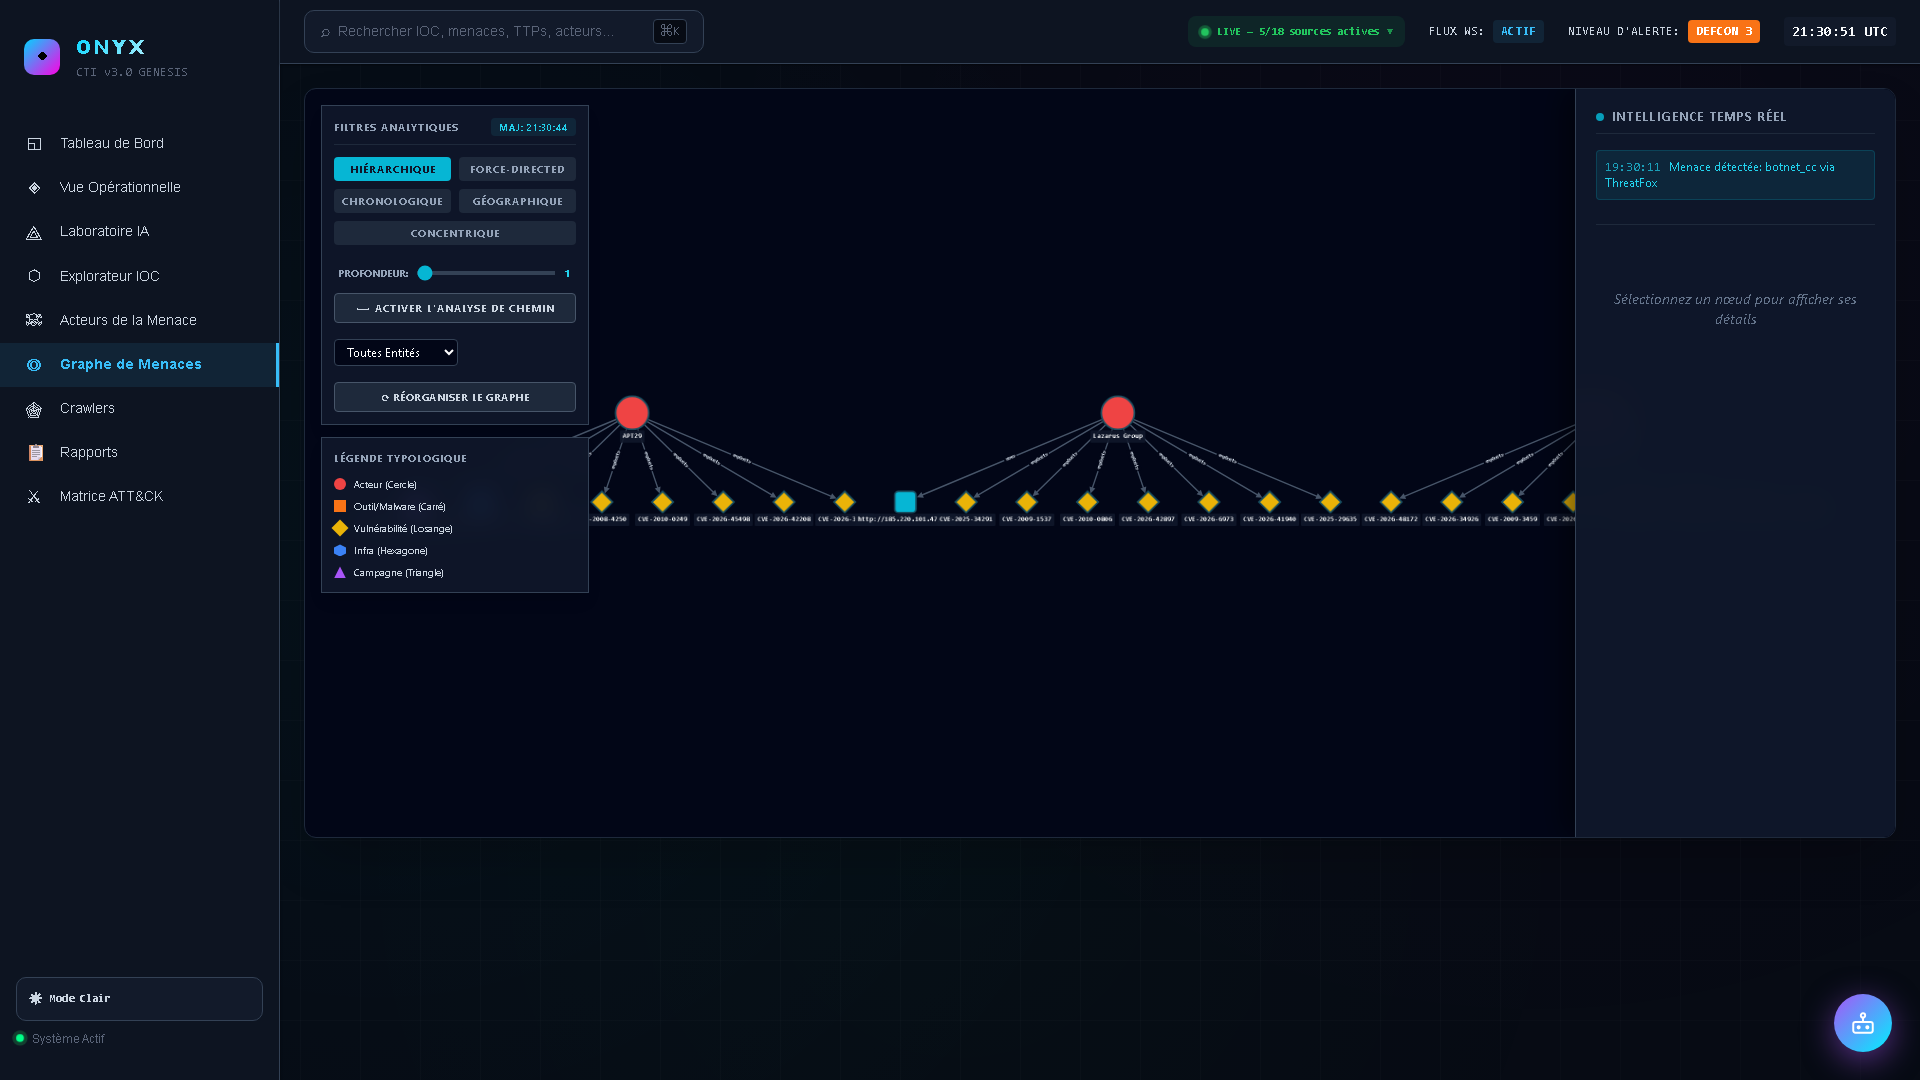
\includegraphics[width=1.0\textwidth, keepaspectratio]{graphe_3d_menace.png}}
    \caption{Graphe de menace Cytoscape.js : topologie relationnelle entre acteurs APT, indicateurs de compromission, vulnérabilités exploitées et infrastructure C2. Disposition hiérarchique (dagre). Les arêtes portent des étiquettes sémantiques STIX~2.1 (\texttt{exploits}, \texttt{uses}, \texttt{attributed-to}).}
    \label{fig:graphe_menace}
\end{figure}

La figure~\ref{fig:graphe_menace} illustre le graphe de menace en conditions opérationnelles. Nous y observons la distribution topologique des entités : les trois acteurs APT (cercles rouges) occupent les positions centrales supérieures, connectés à leurs campagnes respectives (triangles violets) et aux IOC associés (rectangles arrondis cyan et hexagones bleus). Les nœuds partagés entre acteurs (losanges jaunes pour les CVE, carrés orange pour les outils) matérialisent les convergences d'infrastructure détectées par corrélation automatique.

\subsection{Cartographie Géospatiale Tactique}

\subsubsection{Résolution géographique des indicateurs de compromission}

La projection géospatiale des menaces requiert une étape préalable de résolution géographique des adresses IP contenues dans les indicateurs de compromission. Le service \texttt{GeoIPResolver}, implémenté côté serveur en Python, opère selon un algorithme de résolution en cascade à quatre niveaux de dégradation gracieuse (\textit{graceful degradation}) :

\begin{enumerate}
    \item \textbf{Phase 1 --- Table de correspondance exacte} : les adresses IP connues de l'infrastructure de menace sont résolues instantanément via une table de hachage en mémoire (\texttt{\_KNOWN\_IP\_MAP}) pré-chargée avec les coordonnées des serveurs C2 documentés (Bruxelles, Amsterdam, Moscou, Saint-Pétersbourg, etc.). Cette phase offre une latence de résolution de l'ordre de la nanoseconde.
    \item \textbf{Phase 2 --- Base de données MaxMind GeoLite2} : la base de données géographique GeoLite2-City au format MMDB (\textit{MaxMind Database}) est montée en mémoire au démarrage du service. Chaque résolution est effectuée par une recherche binaire dans l'arbre de préfixes CIDR de la base, retournant la latitude, la longitude, le nom du pays et la ville associés au bloc réseau englobant. Cette phase couvre la majorité des adresses IP routables avec une précision au niveau de la ville.
    \item \textbf{Phase 2.5 --- API de géolocalisation externe} : en cas d'échec de la base locale (IP non répertoriée dans la version GeoLite2 installée), une requête HTTP asynchrone est émise vers l'API publique \texttt{ip-api.com} avec un délai d'attente strict de 2~secondes. Cette phase constitue un filet de sécurité pour les blocs IP récemment alloués, non encore couverts par la base locale.
    \item \textbf{Phase 3 --- Correspondance par préfixe déterministe} : si les phases précédentes échouent (IP non résolue ou API indisponible), une table de correspondance par préfixe de premier octet assigne des coordonnées géographiques plausibles (ex. : le préfixe \texttt{194.*} est résolu vers Moscou, \texttt{103.*} vers New Delhi). Cette heuristique, bien que moins précise, garantit qu'aucun événement n'est éliminé du pipeline de visualisation.
    \item \textbf{Phase 4 --- Point zéro (\textit{Null Island})} : en dernier recours absolu, les coordonnées (0.0, 0.0) sont attribuées, signalant visuellement un indicateur non résolu sur l'intersection de l'équateur et du méridien de Greenwich. Ce comportement « \textit{never null} » est une contrainte d'ingénierie critique : il garantit que la fonction \texttt{resolve()} ne retourne jamais une valeur nulle, empêchant les erreurs de type \texttt{NullPointerException} dans la chaîne de rendu Deck.gl en aval.
\end{enumerate}

\subsubsection{Moteur de rendu cartographique : Deck.gl et MapLibre GL}

Le composant \texttt{ThreatMap3D.tsx} implémente la carte tactique en superposant des couches de données vectorielles Deck.gl sur un fond cartographique à tuiles vectorielles fourni par MapLibre GL (thème \textit{CARTO Dark Matter}). L'architecture de rendu est organisée en trois niveaux de détail adaptatifs contrôlés par le facteur de zoom de la caméra :

\begin{itemize}
    \item \textbf{Niveau stratégique} (zoom $< 4$) : les incidents sont agrégés par région continentale (7 régions : Amérique du Nord, Europe Occidentale, Europe Orientale, Moyen-Orient, Asie-Pacifique, Afrique, Amérique Latine). Chaque région est représentée par un \texttt{ScatterplotLayer} dont le rayon est proportionnel au nombre d'incidents et la couleur est déterminée par un score de menace régional calculé algorithmiquement. Les flux inter-régionaux sont matérialisés par un \texttt{ArcLayer} dont les arcs bicolores (rouge-origine vers cyan-cible) relient les régions sources d'attaques aux régions ciblées.
    \item \textbf{Niveau tactique} (zoom $\in [4, 8[$) : les incidents sont désagrégés au niveau national. Chaque pays est représenté par un point dont la couleur signale la présence d'incidents critiques (rouge) ou élevés (orange). Les arcs inter-pays affinent la granularité des flux d'attaques.
    \item \textbf{Niveau opérationnel} (zoom $\geq 8$) : chaque incident individuel est projeté comme un point discret, avec un léger décalage aléatoire des coordonnées ($\pm 1$~degré) pour éviter la superposition des points co-localisés. Ce niveau permet l'inspection détaillée d'un incident spécifique via un clic.
\end{itemize}

Le code suivant présente la configuration des couches Deck.gl pour le niveau stratégique, illustrant le calcul du score de menace régional, la construction du \texttt{ScatterplotLayer} et du \texttt{ArcLayer} inter-régional :

\begin{lstlisting}[language=JavaScript, caption={Configuration des couches Deck.gl : ScatterplotLayer (régions) et ArcLayer (flux d'attaque inter-régionaux) pour le niveau stratégique.}, label={lst:deckgl-layers}]
// Score de menace regional (algorithme composite)
function regionalThreatScore(events) {
  const count = events.length;
  const severityScore = (s) =>
    s === 'critique' ? 5 : s === 'eleve' ? 4
    : s === 'moyen' ? 3 : 2;
  const avgCriticality = count > 0
    ? events.reduce((s, e) =>
        s + severityScore(e.severity), 0) / count
    : 0;
  const diversity = new Set(
    events.map(e => e.threat_type)
  ).size;
  return Math.min(100,
    count * 0.5 + avgCriticality * 20
    + diversity * 5);
}

// Couche 1: Points de menace regionaux
const regionsLayer = new ScatterplotLayer({
  id: 'regions-layer',
  data: scatterData,
  pickable: true,
  opacity: 0.8,
  stroked: true,
  filled: true,
  radiusScale: 10000,
  radiusMinPixels: 10,
  radiusMaxPixels: 60,
  lineWidthMinPixels: 2,
  getPosition: d => d.position,
  getRadius: d => d.size,
  getFillColor: d => d.color,
  getLineColor: [255, 255, 255],
  onHover: i => setHoverInfo(
    i.object ? { ...i, type: 'region' } : null
  )
});

// Couche 2: Arcs d'attaque inter-regionaux
const arcsLayer = new ArcLayer({
  id: 'regions-arcs',
  data: arcData,
  pickable: false,
  getWidth: d => Math.min(d.count, 10),
  getSourcePosition: d => d.source,
  getTargetPosition: d => d.target,
  // Degrade bicolore : rouge (origine) -> cyan (cible)
  getSourceColor: [255, 0, 0, 150],
  getTargetColor: [0, 200, 255, 150],
});
\end{lstlisting}

Nous soulignons trois aspects d'ingénierie de ce moteur cartographique.

\textbf{Score de menace composite.} Le score de menace régional n'est pas un simple compteur d'incidents : il combine trois dimensions --- le volume brut d'incidents (pondéré à 0,5 par événement), la criticité moyenne (pondérée à 20 par point de sévérité) et la diversité typologique (pondérée à 5 par type distinct de menace). Cette formule composite permet de distinguer une région subissant 100 attaques de faible sévérité (score modéré) d'une région subissant 10 attaques critiques multi-vecteurs (score élevé). Le score est plafonné à 100 pour normaliser le rendu chromatique.

\textbf{Arcs bicolores directionnels.} Les arcs de flux d'attaque utilisent un dégradé de couleur asymétrique : rouge à la source (pays attaquant), cyan à la destination (pays ciblé). Cette convention chromatique directionnelle est immédiatement interprétable par l'analyste sans recours à une légende, et les arcs sont filtrés pour n'afficher que les flux comportant au moins 5 incidents, éliminant le bruit visuel des corrélations faibles.

\textbf{Rendu adaptatif par niveau de zoom.} La segmentation en trois niveaux de détail (stratégique, tactique, opérationnel) implémente le principe d'information \textit{à la demande} (\textit{details-on-demand}) de la taxonomie de visualisation de Shneiderman (\textit{overview first, zoom and filter, then details-on-demand}). Cette approche évite la saturation visuelle qui surviendrait si les centaines d'incidents individuels étaient projetés simultanément au niveau mondial.

\subsubsection{Intérêt opérationnel pour l'analyste SOC}

La cartographie géospatiale offre à l'analyste SOC trois capacités d'analyse qui ne sont pas accessibles par les vues tabulaires classiques :

\begin{enumerate}
    \item \textbf{Identification de clusters C2} : la concentration de points d'incidents dans une zone géographique restreinte (ex. : 15 indicateurs résolus dans un périmètre de 50~km autour d'une ville) signale la présence probable d'une infrastructure de commande et de contrôle (C2) mutualisée, exploitable pour des actions de blocage ciblé par plage IP.
    \item \textbf{Attribution géographique} : les arcs de flux d'attaque permettent de visualiser les corridors d'agression dominants. Un arc récurrent reliant l'Europe Orientale à l'Europe Occidentale, avec un score de menace élevé, corrobore les hypothèses d'attribution à des acteurs étatiques spécifiques et informe les décisions de posture défensive.
    \item \textbf{Détection d'anomalies spatiales} : l'apparition soudaine d'un cluster d'incidents dans une région habituellement calme (ex. : pic d'activité en Asie du Sud-Est) constitue un signal faible détectable visuellement avant d'atteindre les seuils d'alerte des systèmes de détection automatisés.
\end{enumerate}

L'interaction entre la carte et les panneaux contextuels enrichit encore cette analyse. Un clic sur un incident ouvre un panneau latéral affichant la criticité, l'horodatage, les IOC associés, l'acteur suspecté et la source OSINT d'origine. Trois actions sont proposées : la recherche d'événements similaires (corrélation par type de menace, acteur ou IOC commun), l'analyse de l'acteur (affichage de la fiche complète avec TTPs MITRE) et la visualisation du flux d'attaque (arc directionnel entre le pays d'origine estimé et le pays cible).

\begin{figure}[H]
    \centering
    \makebox[\textwidth][c]{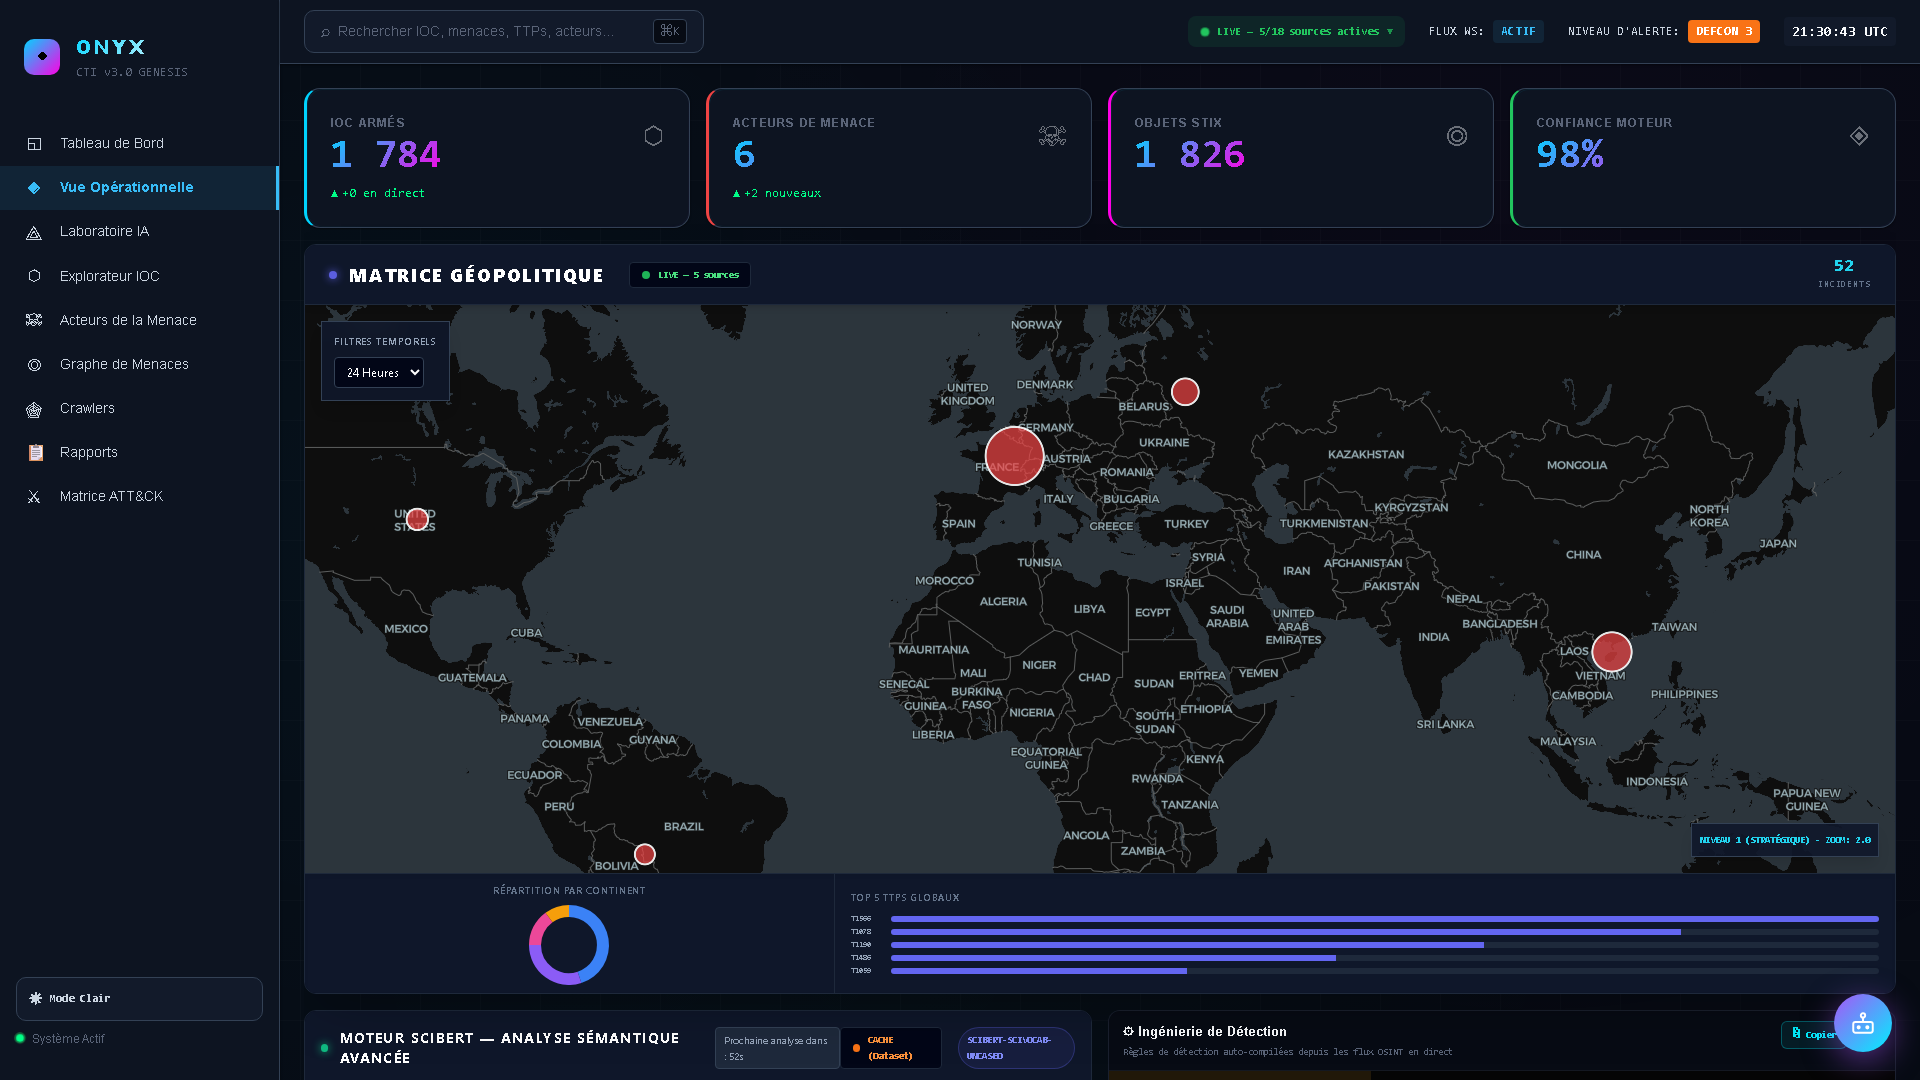
\includegraphics[width=1.0\textwidth, keepaspectratio]{map_geospatiale.png}}
    \caption{Cartographie géospatiale tactique : projection Deck.gl/MapLibre des incidents CTI avec arcs inter-régionaux de flux d'attaque bicolores (rouge-origine, cyan-cible). Fond cartographique CARTO Dark Matter.}
    \label{fig:map_geospatiale}
\end{figure}

La figure~\ref{fig:map_geospatiale} présente la vue cartographique en mode opérationnel. Les points de menace régionaux sont proportionnels au volume d'incidents et colorés selon le score composite. Les arcs bicolores matérialisent les corridors d'attaque dominants entre les zones géopolitiques sources et les cibles. Le panneau supérieur affiche le nombre total d'incidents géo-référencés, le statut de connexion aux sources OSINT et les contrôles de filtrage temporel.
